\section{Simulaciones}

En esta sección se comparan las formas de onda obtenidas con el circuito una vez implementado, con las simulaciones realizadas para el diseño del cargador de baterías.

\subsection{Generador de señal PWM}

Por cuestiones de costo computacional y de falta de un modelo representativo del TL494,
su circuito no fue simulado y se probó directamente en una protoboard,
por lo que no se harán comparaciones con las simulaciones.

Aun así, a continuación se mostrarán las formas de onda mas importantes del circuito implementado,
comparando con las indicadas en la hoja de datos del fabricante.

En la figura \ref{fig:osc_pwm_vout_disconnected} se muestra la forma de onda de la tensión de salida de la etapa de ganancia de corriente, con la fuente de alimentación de 36V desconectada.
Esta debería ser una señal PWM con un período de $8\mu s$ y un ancho de pulso de aproximadamente 16\%

\begin{figure}[H]
    \centering
    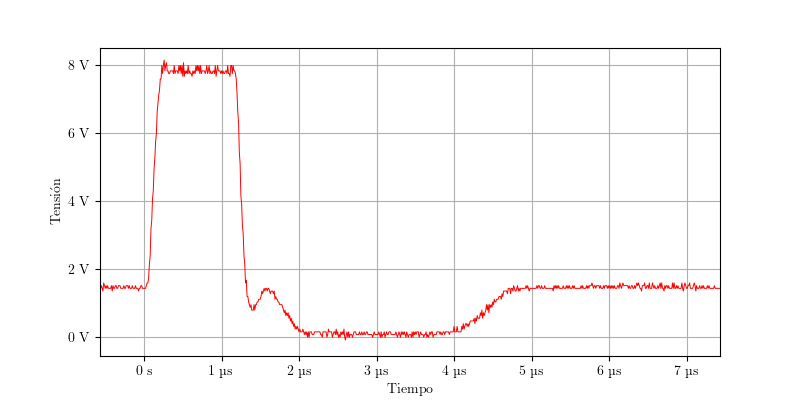
\includegraphics[width=\textwidth]{images/capturas-osciloscopio/TL494/pwm_vout_disconnected.png}
    \caption{Tensión a la salida del TL494 después de la etapa de ganancia de corriente con la fuente de 36V desconectada. Se puede observar que la señal cumple con los requisitos de frecuencia y ancho de pulso}
    \label{fig:osc_pwm_vout_disconnected}
\end{figure}

Se puede observar una tensión de continua de aproximadamente $1.5V$ durante la etapa de apagado del PWM, la cual se debe al capacitor de desacople del circuito primario del driver.

Si se compara la figura \ref{fig:osc_pwm_vout_disconnected} con la \ref{fig:osc_pwm_vout_connected}, la cual muestra la misma forma de onda pero con la fuente de tensión de 36V conectada, se puede observar que la forma de onda es similar, pero se presenta una oscilación de alta frecuencia durante el ciclo de apagado de la señal PWM. Esta oscilación será tratada en la sección %\ref{subsec:oscilaciones}.

\begin{figure}[H]
    \centering
    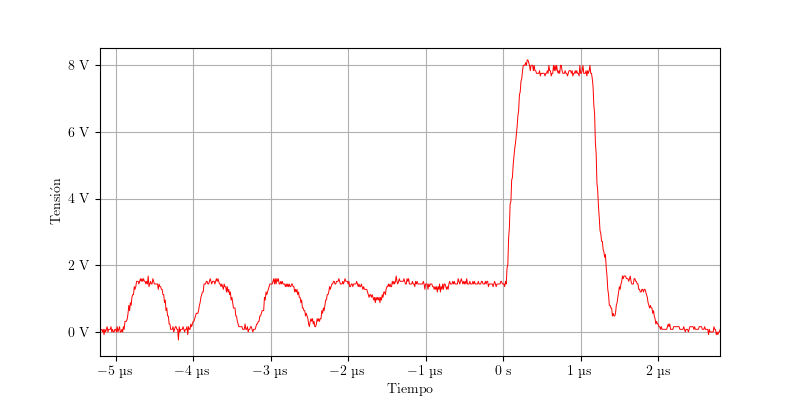
\includegraphics[width=\textwidth]{images/capturas-osciloscopio/TL494/pwm_vout_connected.png}
    \caption{Tensión a la salida del TL494 después de la etapa de ganancia de corriente con la fuente de 36V conectada}
    \label{fig:osc_pwm_vout_connected}
\end{figure}

En las figuras \ref{fig:ct_v} y \ref{fig:dtc_v} se muestran las tensiones en el capacitor $C_t$ y el terminal DTC del TL494 respectivamente.

\begin{figure}[H]
    \centering
    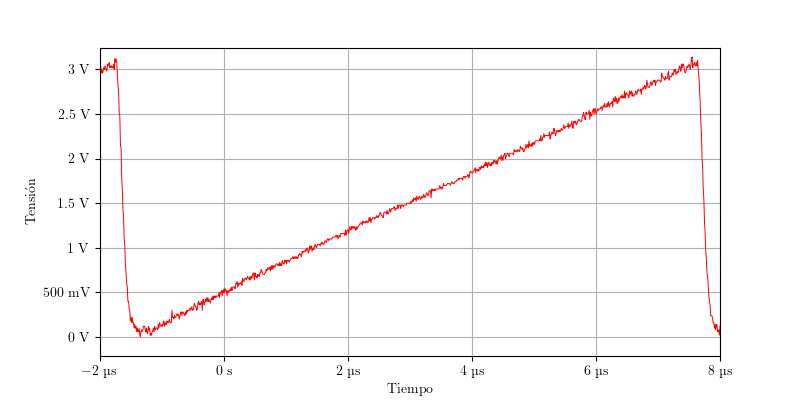
\includegraphics[width=\textwidth]{images/capturas-osciloscopio/TL494/Ct_v.png}
    \caption{} %COMPLETAR
    \label{fig:ct_v}
\end{figure}

% La forma de onda de Ct es la esperada, pero la de DTC?

\begin{figure}[H]
    \centering
    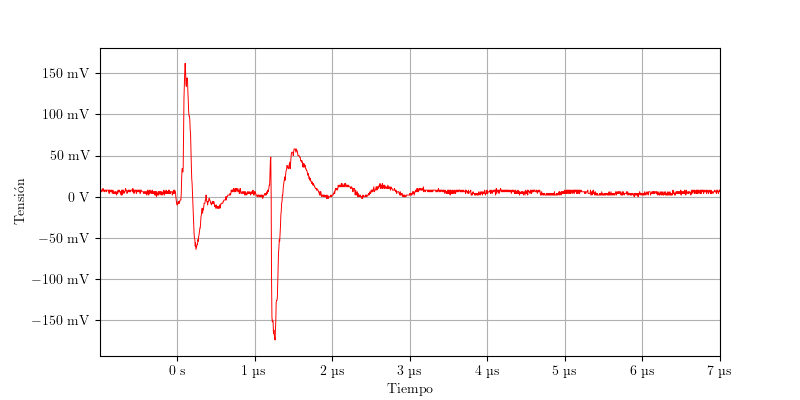
\includegraphics[width=\textwidth]{images/capturas-osciloscopio/TL494/DTC_v.png}
    \caption{} %COMPLETAR
    \label{fig:dtc_v}
\end{figure}

% 1) Señal PWM

% Se toma la salida por el colector de los transistores del circuito integrado. 
% Su forma de onda son pulsos rectangulares. 
% Amplitud: 0V a Vdrv dados por la tensión de alimentación.
% Frecuencia de 125kHz dada por el capacitor Ct=1nF y $Rt=8k\Omega$ mediante el potenciómetro. 
% Tiempo de encendido: permite controlar el ciclo de trabajo mediante un potenciómetro. 
% Esta señal se mide en 3 condiciones diferentes: 
% A) Sin el convertidor forward conectado
% B) Con el convertidor forward conectado pero sin su alimentación de 36V
% C) Con el convertidor forward conectado y alimentado

% 2) Diente de Sierra 

% Tensión en el capacitor Ct. 

% 3) Tensión en el puerto DTC 

\subsection{Etapa de ganancia de corriente}

Esta etapa se encarga de aumentar la corriente de salida del TL494 para alimentar las compuertas de los MOSFETs del convertidor.
Fue agregada para mejorar la forma de onda de la señal PWM, ya que la carga que generaba el circuito sobre el TL494 era muy alta y, a demas de distorsionarse la forma de onda, la tensión caía demasiado, lo que causaba que los MOSFETs no se saturaran, y por ende aumentara demasiado la temperatura de los mismos.

Consta de dos transistores BJT % COMO SE LLAMA ESTA CONFIGURACION???? No encuentro nada 

En las figuras \ref{fig:pwm_iout_sin_bjt} y \ref{fig:pwm_iout_con_bjt} puede observarse la corriente de salida del TL494 antes y después de agregar la etapa de ganancia de corriente, respectivamente.

\begin{figure}[H]
    \centering
    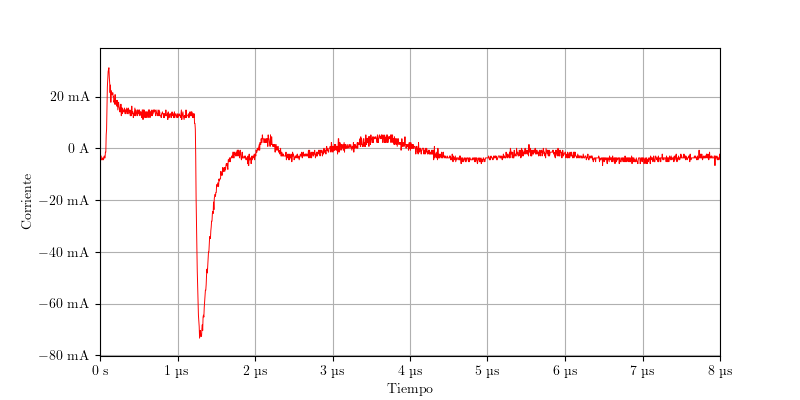
\includegraphics[width=\textwidth]{images/capturas-osciloscopio/TL494/pwm_iout_sin_bjt.png}
    \caption{Corriente a la salida del TL494 sin colocar la etapa intermedia de ganancia de corriente}
    \label{fig:pwm_iout_sin_bjt}
\end{figure}

\begin{figure}[H]
    \centering
    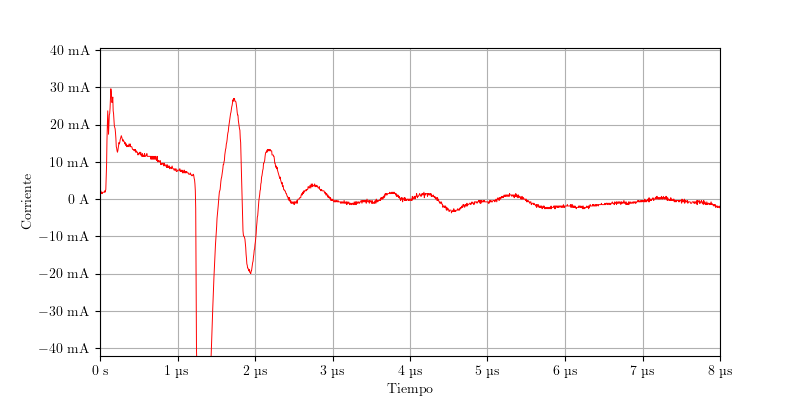
\includegraphics[width=\textwidth]{images/capturas-osciloscopio/BJT/bjt-iin-con-etapa.png}
    \caption{Corriente a la salida del TL494 con la etapa intermedia de ganancia de corriente}
    \label{fig:pwm_iout_con_bjt}
\end{figure}

Puede observarse que las oscilaciones aumentan. %WHAT?

La funcion más importante de esta etapa es la de mejorar la forma de onda de la señal PWM, que al comparar las figuras \ref{fig:osc_pwm_vout_disconnected} y \ref{fig:pwm_vout_sin_bjt} se puede observar que se ha mejorado considerablemente.

\begin{figure}[H]
    \centering
    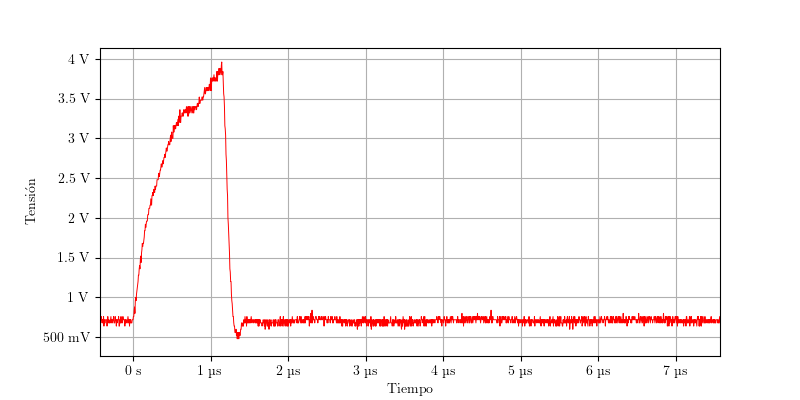
\includegraphics[width=\textwidth]{images/capturas-osciloscopio/TL494/pwm_vout_sin_bjt.png}
    \caption{Tensión a la salida del TL494 sin colocar la etapa intermedia de ganancia de corriente}
    \label{fig:pwm_vout_sin_bjt}
\end{figure}

% 1) Corriente sin la etapa 
% DONE

% 2) Corriente de entrada y de salida con la etapa

% 3) Tensión a la salida sin la etapa
% DONE

% 3) Tensión a la salida con la etapa
% DONE

% Hay que ver eso de las oscilaciones en la corriente

\subsection{Driver}

Debido a la configuración de conversor elegida, se requiere un driver para controlar el MOSFET cuyo terminal de \textit{source} no está a tierra. Se optó por un driver con transformador acoplador ya que provee aislación galvánica entre el circuito de control y el circuito de potencia \cite{gatedrivers}.

En las figuras \ref{fig:driver_vout_connected} y \ref{fig:driver_vout_disconnected} se muestra la salida del driver con y sin el convertidor energizado, respectivamente.
Se puede ver que también están presentes las oscilaciones de alta frecuencia que se observan en la salida del TL494.

\begin{figure}[H]
    \centering
    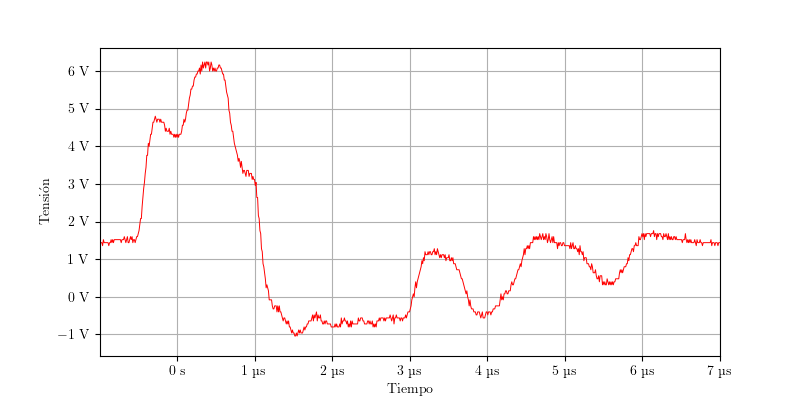
\includegraphics[width=\textwidth]{images/capturas-osciloscopio/DRIVER/driver_vout_connected.png}
    \caption{Tensión a la salida del driver con la fuente de 36V conectada}
    \label{fig:driver_vout_connected}
\end{figure}
% HAY QUE ORDENAR ESTAS 2
\begin{figure}[H]
    \centering
    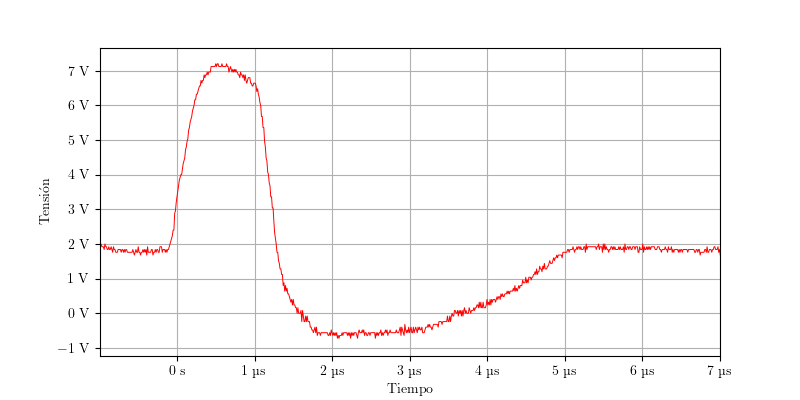
\includegraphics[width=\textwidth]{images/capturas-osciloscopio/DRIVER/driver_vout_disconnected.png}
    \caption{Tensión a la salida del driver con la fuente de 36V desconectada}
    \label{fig:driver_vout_disconnected}
\end{figure}

En la figura \ref{fig:driver_expected_waveforms} se muestran algunas formas de onda del circuito del driver con las que se hicieron comparaciones para verificar su correcto funcionamiento.

\begin{figure}[H]
    \centering
    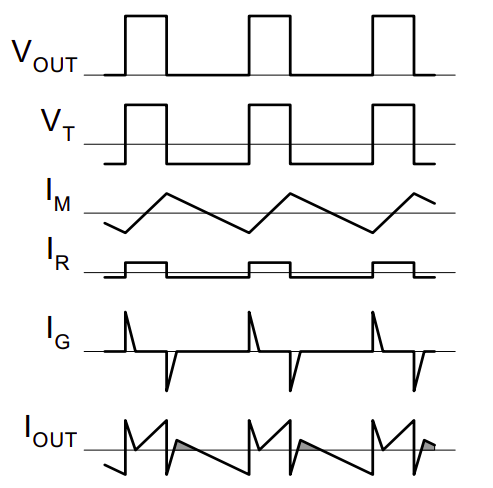
\includegraphics[width=0.7\textwidth]{images/driver_expected_waveforms.png}
    \caption{Formas de onda esperadas de distintas señales del driver \cite{gatedrivers}}
    \label{fig:driver_expected_waveforms}
\end{figure}

%Falto medir la mayoría de esto?
% 1) Tensiones en el transformador de señal 

    % Forma de onda: Rectangular 
    % Amplitud: -Vc a Vdrv-Vc 
    % Son iguales dada la relación 1:1 del transformador. 

% 2) Tensión Gate del MOSFET high side % Sería vout del driver?
% DONE

    % Forma de onda: Rectangular 
    % Amplitud: -Vd a Vdrv-Vd
    % Vd: Tensión en el diodo del secundario

% 3) Corriente de salida % FALTA MEDIR LAS CORRIENTES CON LA PCB

    % Compuesta por:

    % A) Corriente magnetizante

        % Forma de onda: triangular
        % Se mide en la Rc del primario. 

    % B) Corriente por Rgs

        % Forma de onda: rectangular

    % C) Corriente por Gate

        % Forma de onda: diente de sierra invertida y espejada con tiempo muerto 

\subsection{Convertidor Forward Doble Switch}

% Agregar intro

% 1) Vgs de ambos MOSFETs %Ya se midió en otros lados

% 2) Vds de ambos MOSFETs

En las figuras \ref{fig:vds_high} y \ref{fig:vds_low} se muestran las tensiones en los terminales \textit{drain} y \textit{source} de los MOSFETs del convertidor forward doble switch.
Para comparar, se muestra en la figura \ref{fig:vds_simulation} la tensión $V_{DS}$ del MOSFET low side simulada en LTSpice. Idealmente, las formas de onda en ambos transistores son iguales.

\begin{figure}[H]
    \centering
    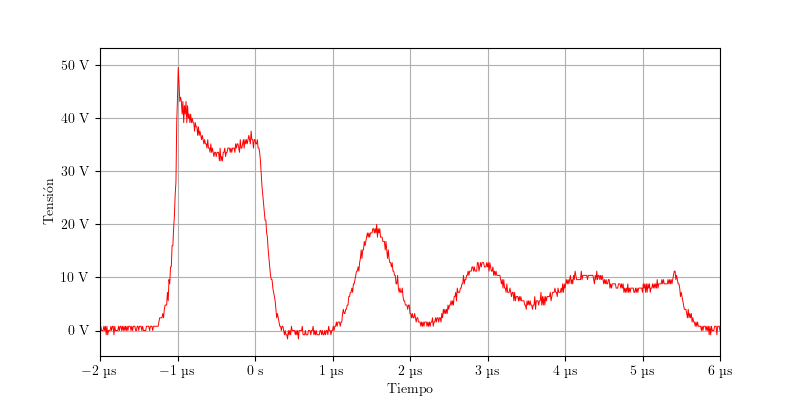
\includegraphics[width=0.7\textwidth]{images/capturas-osciloscopio/MOSFET/vds-high.png}
    \caption{Tensión $V_{DS}$ en el MOSFET high side}
    \label{fig:vds_high}
\end{figure}

\begin{figure}[H]
    \centering
    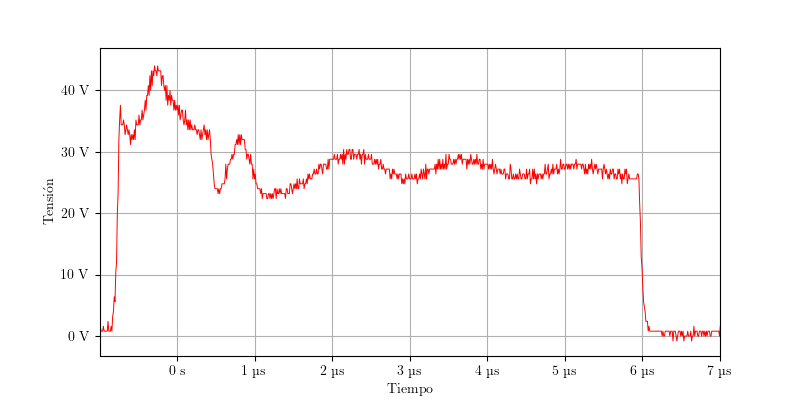
\includegraphics[width=0.7\textwidth]{images/capturas-osciloscopio/MOSFET/vds-low.png}
    \caption{Tensión $V_{DS}$ en el MOSFET low side}
    \label{fig:vds_low}
\end{figure}

% \begin{figure}[H]
%     \centering
%     \includegraphics[width=0.7\textwidth]{images/vds_sim.png}
%     \caption{Tensión $V_{DS}$ en el MOSFET low side simulado en LTspice}
%     \label{fig:vds_low}
% \end{figure}

% 3) Idrain de ambos MOSFETs

% 4) Tensiones en el E70

% 5) Corriente en el primario

    % Medir la componente continua. 

% 6) Caída de tensión en los diodos

% 7) Corriente en el inductor junto con su ripple

% 8) Corriente de salida junto con su ripple 

    % Idealmente medir 1A-1.6A del modo elegido. 

% 9) Tensión de salida junto con su ripple 

\subsubsection{Simulación de distintos modelos de batería}
Para que las simulaciones permitan obtener resultados fiables se buscó un modelo apropiado para la batería.
El primer modelo consta de una resistencia variable a partir de los datos obtenidos de los ensayos. 
Este componente representa la resistencia equivalente que presenta la batería,
que es responsable de la caída de tensión instantánea que se produce ante un escalón en la intensidad demandada.

El siguiente modelo propuesto añade un capacitor de muy alto valor en serie con la resistencia variable,
el cual representa la capacidad de almacenar carga de la batería.
El modelo actual es un modelo dinámico donde los valores de los componentes no son fijos,
sino que dependen de las condiciones de funcionamiento de la batería: estado de carga y funcionamiento en carga o descarga.

El circuito de la izquierda modela la resistencia interna de la batería y el comportamiento transitorio ante distintas cargas.
Por otro lado, el circuito de la derecha modela la capacidad de almacenamiento de energía de la batería y la carga almacenada durante los procesos de carga o descarga \cite{modelo_bateria_1}.

\begin{figure}
    \centering
    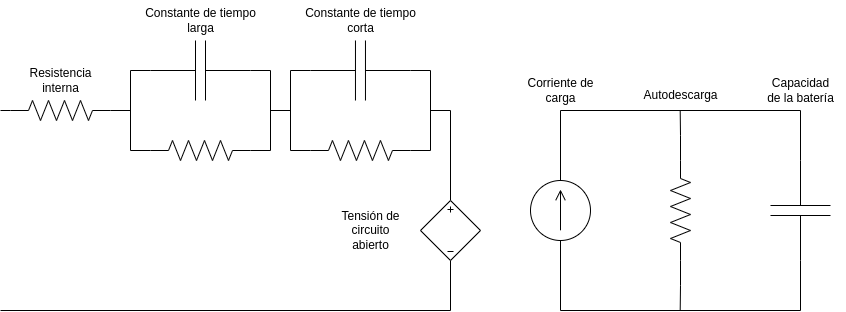
\includegraphics[width=\textwidth]{images/modelo_bateria.png}
    \caption{Modelo final de batería utilizado}
    \label{fig:bateria_3}
\end{figure}

Respecto al segundo modelo se agregan los siguientes componentes:
\begin{itemize}
    \item Los bloques compuestos por una resistencia y un capacitor en paralelo, que modelan la capacidad en los electrodos de las celdas y
    la resistencia no lineal entre electrodos y electrolito.
    En conjunto modelan las constantes de tiempo (corta y larga) de la respuesta transitoria de la tensión en la batería \cite{modelo_bateria_2}.
    \item La fuente de tensión controlada por tensión, que representa la dependencia no lineal entre el estado de carga ($SOC$)
    y la tensión de circuito abierto($V_{OC}$) dependiente del $SOC$.
    \item La fuente de corriente controlada por corriente, representa la corriente de carga que modifica el $SOC$.
\end{itemize}
La tensión que existe en el circuito secundario ($V_{SOC}$) se normaliza de forma que $V_{SOC}=1V$ equivale al $SOC (100\%)$.
La resistencia en paralelo modela la autodescarga de la batería.
